% !TEX TS-program = pdflatex
% !TEX encoding = UTF-8 Unicode

% This is a simple template for a LaTeX document using the "article" class.
% See "book", "report", "letter" for other types of document.

\documentclass[11pt]{article} % use larger type; default would be 10pt

\usepackage[utf8]{inputenc} % set input encoding (not needed with XeLaTeX)
\usepackage{amsmath}
\usepackage{graphicx}
\usepackage[backend=biber]{biblatex}
\addbibresource{references.bib}

\numberwithin{equation}{section} % number within sections
% \usepackage[parfill]{parskip} % new line without indent

%%% Examples of Article customizations
% These packages are optional, depending whether you want the features they provide.
% See the LaTeX Companion or other references for full information.

%%% PAGE DIMENSIONS
\usepackage{geometry} % to change the page dimensions
\geometry{a4paper} % or letterpaper (US) or a5paper or....
% \geometry{margin=2in} % for example, change the margins to 2 inches all round
% \geometry{landscape} % set up the page for landscape
%   read geometry.pdf for detailed page layout information

\usepackage{graphicx} % support the \includegraphics command and options

% \usepackage[parfill]{parskip} % Activate to begin paragraphs with an empty line rather than an indent

%%% PACKAGES
\usepackage{booktabs} % for much better looking tables
\usepackage{array} % for better arrays (eg matrices) in maths
\usepackage{paralist} % very flexible & customisable lists (eg. enumerate/itemize, etc.)
\usepackage{verbatim} % adds environment for commenting out blocks of text & for better verbatim
\usepackage{subfig} % make it possible to include more than one captioned figure/table in a single float
% These packages are all incorporated in the memoir class to one degree or another...

%%% HEADERS & FOOTERS
\usepackage{fancyhdr} % This should be set AFTER setting up the page geometry
\pagestyle{fancy} % options: empty , plain , fancy
\renewcommand{\headrulewidth}{0pt} % customise the layout...
\lhead{}\chead{}\rhead{}
\lfoot{}\cfoot{\thepage}\rfoot{}

%%% SECTION TITLE APPEARANCE
\usepackage{sectsty}
\allsectionsfont{\sffamily\mdseries\upshape} % (See the fntguide.pdf for font help)
% (This matches ConTeXt defaults)

%%% ToC (table of contents) APPEARANCE
\usepackage[nottoc,notlof,notlot]{tocbibind} % Put the bibliography in the ToC
\usepackage[titles,subfigure]{tocloft} % Alter the style of the Table of Contents
\renewcommand{\cftsecfont}{\rmfamily\mdseries\upshape}
\renewcommand{\cftsecpagefont}{\rmfamily\mdseries\upshape} % No bold!

%%% END Article customizations

%%% The "real" document content comes below...

\title{Development of a Cost-Effective 1kN Liquid-Fueled Rocket Propulsion System}
\author{%
	Jason Chen, Project Caelus 501(c)(3)  \\
	\large contact@projectcaelus.org}
%\date{} % Activate to display a given date or no date (if empty),
         % otherwise the current date is printed 

\begin{document}
\maketitle

\section{Pipe Dimension Calculation}

The following section describes the theoretical process used to dimensionalize the prelimiary plumbing framework in preparation for the first static cold flow test. By definition, these calculations are purely speculatory and are only used for the initial design process. The purpose of the cold flow test is to verify these parameters, and consequently adjust these parameters to better fit the system requirements.

\subsection{Assumptions} \label{sec:assumptions}

To simplify the rigorous analysis and optimization processes often associated with viscous pipe flow, a couple of assumptions are applied in the following section to both shorten the development timeline and to avoid unecessarily complex or expensive methods outside of the scope of a high school amateur rocketry program. They are as follows:
\begin{enumerate}
\item Flow is driven by both pressure and gravity.
\item Pipe is circular and is of constant cross-sectional area. \label{itm:constant-area}
\item No swirl, circumferential variation, or entrance effects.
\item No shaft-work or heat-transfer effects. \label{itm:heat-effects}
\item A simplified steady-flow energy equation due to Assumption \ref{itm:heat-effects}.
%\item Flow is fully developed (minimal boundary-layer effects).

\end{enumerate}
\subsection{The Reynolds Transport Theorem}
We can begin by introducing the concept of control-volume analysis \textemdash{} a powerful approach to solving fundamental fluid mechanics problems \textemdash{} in which a mathematical abstraction is employed to generate mathematical models of physical systems. That is, in an inertial frame of reference, the \textit{control volume} is a volume fixed in space or moving with constant velocity with the fluid flow. The surface enclosing the control volume is referred to as the \textit{control surface}. To convert a system analysis to a control-volume analysis, we must shift our perspective such that our mathematics apply to a specific region rather than to individual bodies. This process is called the \textit{Reynolds Transport Theorem}, and allows us to study certain properties (e.g. angular momentum $L$, enthalpy $h$, etc.) crossing the boundaries of the region. Essentially, we need to relate the time derivative of a system property of that property within a certain region.
\begin{figure}[h] \label{fig:control-types}
\centering
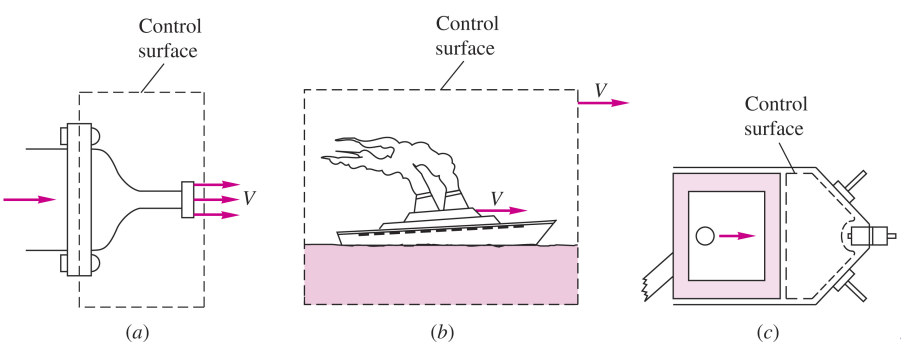
\includegraphics[scale=0.5]{control_types}
\caption{Fixed, moving, and deformable control volumes: (a) fixed control volume for nozzle stress analysis; (b) control volume moving at ship speed for drag force analysis; (c) control volume deforming within cylinder for transient pressure variation analysis.}
\end{figure}

The desired conversion formula differs slightly according to whether the control volume is fixed, moving, or deformable, but for the purposes of our application, we'll be focusing on a fixed control volume. The fixed control volume in Figure \ref{fig:control-types}$a$ encloses a stationary region of interest to a nozzle designer. The control surface is an abstract concept that does not hinder the flow in any way. It slices through the jet leaving the nozzle, circles around through the surrounding (ambient) atmosphere, and slices through the flange bolts and the fluid within the nozzle \cite{fluid-mechanics}.

This particular control volume exposes the stresses in the flange bolts, which contribute to applied forces in the momentum analysis. In this sense, the control volume resembles the \textit{free-body} concept, which is often applied in solid-mechanics analysis \cite{fluid-mechanics}.
\begin{figure}[h] \label{fig:control-volume}
\centering
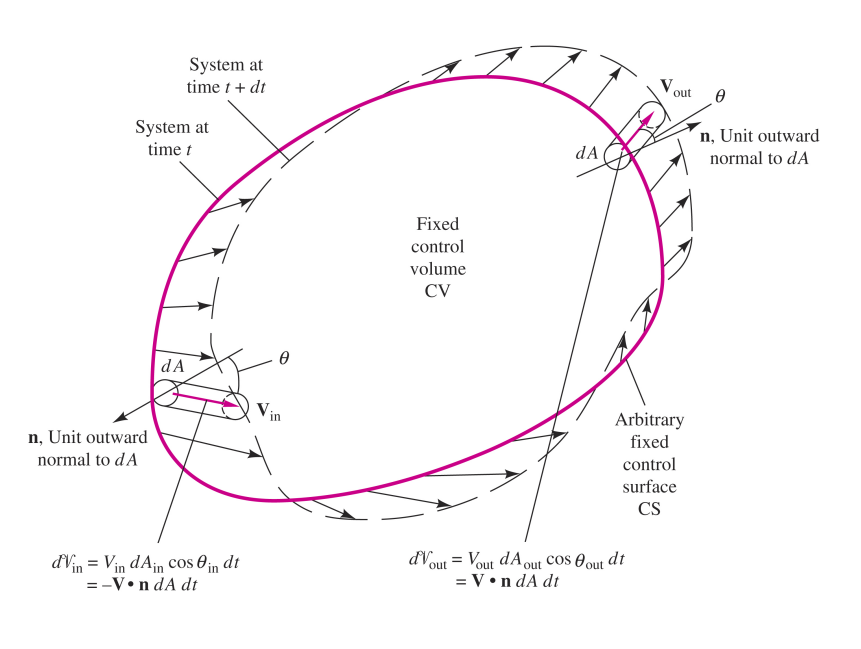
\includegraphics[scale=0.5]{control_volume}
\caption{An arbitrary fixed control volume with an arbitrary flow pattern.}
\end{figure}

Figure \ref{fig:control-volume} shows a generalized fixed control volume with an arbitrary flow pattern passing through. In general, each differential $dA$ of surface will have a different velocity vector $\vec{V}$ making a different angle $\theta$ with the local normal to $dA$. This gives us the general Reynolds transport theorem equation for an arbitrary fixed control volume:
\begin{equation} \label{eq:long-rtt}
\frac{d}{dt}(B_{syst}) = \frac{d}{dt} \left( \int_{CV} \beta \rho\, d\vartheta \right) + \int_{CS} \beta \rho\, cos\theta\, dA_{out} - \int_{CS} \beta \rho\, cos\theta\, dA_{in}
\end{equation}
Asserting the property $B$ to be either mass, momentum, angular momentum, or energy, all basic laws can be rewritten in control-volume form. Note that all three control volume integrals are a function of the intensive propery $\beta$, and since the control volume is fixed in space, the elemental volumes $d\vartheta$ do not vary with time, and thus the time derivative of the volume integral disappears unless $\beta$ or $\rho$ varies with time (unsteady flow) \cite{fluid-mechanics}.

However, realizing that if $\vec{n}$ is defined as the \textit{outward} normal unit vector everywhere on the control surface, then $\vec{V} \cdot \vec{n} = V_{n}$ for outflow and $\vec{V} \cdot \vec{n} = -V_{n}$ for inflow. Therefore, the flux terms can be combined and Equation \ref{eq:long-rtt} can be rewritten as
\begin{equation} \label{eq:short-rtt}
\frac{d}{dt}(B_{syst}) = \frac{d}{dt} \left( \int_{CV} \beta \rho\, d\vartheta \right) + \int_{CV} \beta \rho(\vec{V} \cdot \vec{n})\, dA
\end{equation}
We are now able to apply the principles of conservation of mass to the Reynolds transport theorem by setting the arbitrary variable $B$ equal to mass, and $\beta = dm/dm =1$. Equation \ref{short-rtt} becomes
\begin{equation}
\left( \frac{dm}{dt} \right)_{syst} = 0 = \frac{d}{dt} \left( \int_{CV} \rho\, d\vartheta \right) + \int_{CS} \rho(\vec{V_{r}} \cdot \vec{n})\, dA
\end{equation}
This is the integral mass-conservation law for a deformable control volume. Adapting this for a fixed control volume and simplying gives
\begin{equation} \label{eq:mass-conservation-law}
\int_{CV} \frac{\partial \rho}{\partial t}\, d\vartheta + \int_{CS} \rho(\vec{V} \cdot \vec{n})\, dA = 0
\end{equation}
Finally, knowing that we are dealing with steady, incompressible flow through the control volume ($\partial \rho/ \partial t = 0$), Equation \ref{eq:mass-conservation-law} reduces to
\begin{equation}
\int_{CS} \rho(\vec{V} \cdot \vec{n})\, dA = 0
\end{equation}
This equation explicitly states that in steady flow, the mass flows entering and exitting the control volume are exactly equal, while neglecting sources or sinks of mass which might be embedded in the control volume.

\subsection{Flow in a Circular Pipe}

Given the simplifying assumptions mentioned in Section \ref{sec:assumptions}, we can begin with the classic case of Bernoulli's Equation:
\begin{equation} \label{eq:bernoulli}
p + \frac{1}{2} \rho V^{2} + \rho g z = constant
\end{equation}
where $p$ is the pressure, $\rho$ is density, $V$ is the total velocity, $z$ is elevation, and $g$ represents gravitational acceleration. It gives insight into the balance between pressure, velocity, and elevation by assuming that the two points in question lie on a streamline, the fluid is incompressible, the flow is steady and inviscid, and there is no friction. Although useful for some applications, it is not adequate for designing robust piping systems which will in actuality encounter such effects.

The addition of a \textit{head loss} term, denoted as $h_{f}$, is the first step in introducing a viscous term into an otherwise inviscid equation. Head loss can simply be thought of as an additional pressure loss in the system due to viscous effects, a sudden expansion/contraction, and/or obstructions to its path such as pipe elbows, bends, valves, etc. This can be done by first realizing that the continuity (conservation of mass) equation, when an arbitrary fixed control volume has only a number of one-dimensional inlets and outlets and when the flow within the control volume is steady ($dp/dt = 0$), can be written simply as
\begin{equation} \label{eq:conservation-of-mass}
\int_{CS} \rho(\vec{V} \cdot \vec{n}) dA = 0
\end{equation}
%%% CHANGE THIS
Equation \ref{eq:conservation-of-mass} above refers to the following figure (see References):
%%%
Due to Assumption \ref{itm:constant-area}, Equation \ref{eq:conservation-of-mass} reduces to 
\begin{equation}
Q_{1} = Q_{2} = constant
\end{equation}
\begin{equation}
V_{1} = \frac{Q_{1}}{A_{1}} = V_{2} = \frac{Q_{2}}{A_{2}}
\end{equation}
Bernoulli's Equation (Equation \ref{eq:bernoulli}, in combination with the steady-flow energy equation) can thus be reduced and rearranged into
\begin{equation}
E =mc^{2}
\end{equation}
We can begin by introducing the dimensionless Darcy friction factor $f$ as a baseline relationship between roughness and pipe resistance:
\begin{equation} \label{eq:darcy-friction}
\frac{8 \tau_{w}}{\rho V^{2}} = f = F(Re_{d}, \frac{\epsilon}{d})
\end{equation}
where $\tau_{w}$ depicts the wall shear stress, $\rho$ is density, $V$ is the mean velocity, and $F$ represents a later-defined function between the Reynold's Number $Re_{d}$ and the average pipe roughness to diameter ratio $\frac{\epsilon}{d}$ (also known as relative roughness).

Using Equation \ref{eq:darcy-friction} and the wall shear stress equation (see References), we obtain the desired expression for finding pipe-head loss, also known as the Darcy-Weisbach equation. It is valid for duct flows of any cross section and any Reynold's Number
\begin{equation} \label{eq:darcy-weisbach}
h_{f} = f{\frac{L}{d}}{\frac{V^{2}}{2{g}}}
\end{equation}
where $h_{f}$ represents the head loss factor as a function of the dimensionless Darcy friction factor $f$, $L$ is the length of the pipe, and $g$ is equal to one standard Earth gravity.


\subsection{Iterative Diameter Calculation}
\subsection{Example Calculation}
\subsubsection{Determining Head Loss and Pressure Drop Using the Moody Chart}

\subsection{Units and Symbols} \label{sec:units}
All units are implied with accordance to the Metric system (seconds, kilograms, Pascals, etc.), but are defined explicity along with common Greek symbols below for ease-of-use:
\begin{itemize}%[\label{}]
\item $Q$ = volumetric flow rate, $m^{3}/s$
\item $u$ = velocity, $m/s$ 
\item $u(r), V$ = local mean velocity, $m/s$ 
\item $u_{max}$ = local maximum velocity, $m/s$ 
\item $\mu$ = dynamic viscosity, $\frac{kg}{m \cdot s}$ or $Pa \cdot s$
\item $\nu$ = kinematic viscosity, $m^{2}/s$
\item $R$ = radius, $m$

\end{itemize}
As \textcite{fluid-mechanics} says, make sure to check your \textcite{pipe-roughness}!
\printbibliography
\end{document}
